\graphicspath{{assets/conclusions/}}


\section{Conclusion}
    %%
    \begin{frame}{Summary - Takeaways}
        \begin{itemize}
            \item Quantum computing offers interesting perspectives in several fields (Machine Learning, Cryptography, Quantum Internet, Business, ...)
            \item It's too early to put anything in \alert{production}, but there's a lot of \alert{research} in the field
            \item Quantum computing will be a \alert{parallel} form of computing with classical computing — not a \alert{replacement}
            \item Every business should get prepared in advance for it and its potentially \alert{outbreaking} results
        \end{itemize}        
    \end{frame}

    %%
	\begin{frame}{Summary}
    	All the material used for this presentation is available at the following link:
		
    	\begin{center}
    		\url{https://github.com/mspronesti/talk-qml-amadeus}
    	\end{center}
    	\begin{center}\ccbysa\end{center}
    \end{frame}

       %%
	\begin{frame}{Summary}
    	% Qlearnkit is available at:
    	\begin{minipage}[c]{0.2\textwidth}
    	\centering
			
\includegraphics[width=0.5\linewidth]{gh_logo}
		\end{minipage}
		\begin{minipage}[c]{0.7\textwidth}
    		\url{https://github.com/mspronesti/qlearnkit}
		\end{minipage}
    	
    	
    	% And can be installed with:
    	 \vspace{\abovedisplayskip}
    	\begin{minipage}[c]{0.2\textwidth}
    	\centering
			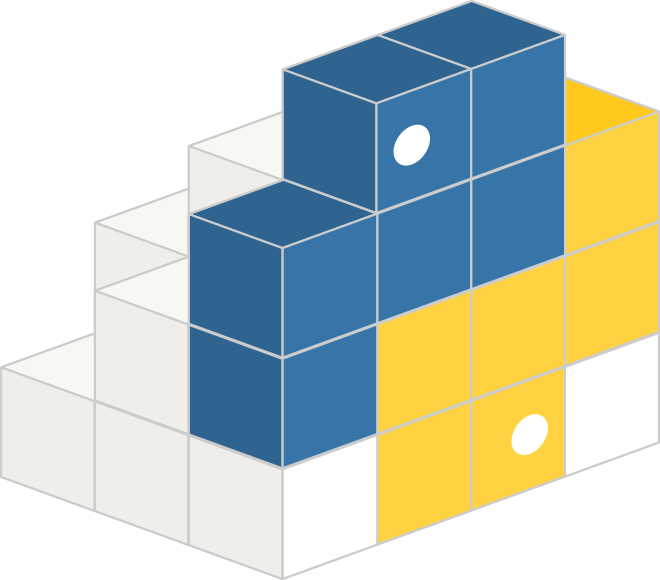
\includegraphics[width=0.5\linewidth]{pypilogo}
		\end{minipage}
		\begin{minipage}[c]{0.7\textwidth}
                \texttt{\$ pip install qlearnkit}
		\end{minipage}
	
	
		  \vspace{\abovedisplayskip}
		\begin{minipage}[c]{0.2\textwidth}
			\centering
			
\includegraphics[width=0.6\linewidth]{docs}
		\end{minipage}
		\begin{minipage}[c]{0.7\textwidth}
			\url{https://mspronesti.github.io/qlearnkit}
		\end{minipage}
		
    	\begin{center}\ccbysa\end{center}
    \end{frame}